\subsection{紧支集连续函数}

定义 1. --- 设 X 是一个拓扑空间，设 E 或者是 \(\overline{R}\) ，或者是 R 上的一个向量空间，并设 f 是 X 到 E 中的一个映射。X 中使 \(\mathbf{f}(x)=0\) 在 X-S 上成立的最小闭集 S （换句话说，一切 \(x\in X\) 中使 \(\mathbf{f}(x)\neq0\) 者所成的集在 X 中的闭包）称为 f 的支集，记作 Supp(f)。

设 X 是一个局部紧空间，E 是 R 或 C 上的一个拓扑向量空间；回忆一下，\(\mathcal{C}(X;E)\) 表示 X 到 E 中的连续映射所成的向量空间；当 E=R 或 E=C 时，若不致引起混淆，我们将省略此记号中的 E。我们将用 \(\mathcal{K}(X;E)\) 表示 \(\mathcal{C}(X;E)\) 中由具有紧支集的连续映射组成的子空间；对 X 的每个子集 A，我们用 \(\mathcal{C}(X,A;E)\) （相应地，\(\mathcal{K}(X,A;E)\) ）表示 \(\mathcal{C}(X;E)\) （相应地，\(\mathcal{K}(X;E)\) ）中由满足 Supp(f) ⊂ A 的映射 f 组成的子空间。若 E=R 或 E=C，在不致引起混淆时，我们写 \(\mathcal{K}(X)\) （相应地，\(\mathcal{K}(X,A)\) ）以代替 \(\mathcal{K}(X;\mathbf{R})\) 或 \(\mathcal{K}(X;\mathbf{C})\) （相应地，\(\mathcal{K}(X,A;\mathbf{R})\) 或 \(\mathcal{K}(X,A;\mathbf{C})\) ）；我们用 \(\mathcal{K}_{+}(X)\) 表示由函数 \(\geqslant0\) （属于 \(\mathcal{K}(X;\mathbf{R})\) ）组成的带顶点的凸锥。

对 X 的每个紧子集 K，空间 \(\mathcal{K}(X,K;E)\) 可以等同于连续函数空间 \(\mathcal{C}(K;E)\) 的一个子空间（即 K 到 E 中的连续映射中在 K 的边界 \(^{1}\) 上为零的那些所成的子空间）。当 \(\mathcal{C}(K;E)\) 赋以 K 中的一致收敛拓扑时，\(\mathcal{K}(X,K;E)\) 是 \(\mathcal{C}(K;E)\) 的一个闭子空间。特别地，若 E 是一个 Fréchet 空间（相应地，Banach 空间），则 \(\mathcal{K}(X,K;E)\) 亦然，因为若 E 的拓扑由半范数 \(p_{n}\) （相应地，范数 \(x \mapsto \|x\|\) ）定义，则 \(\mathcal{K}(X,K;E)\) 的拓扑由半范数 \(\mathbf{f} \mapsto \sup_{x \in K} p_n(\mathbf{f}(x))\) （相应地，范数 \(\mathbf{f} \mapsto \sup_{x \in K} \| \mathbf{f}(x) \|\) ，记作 \(\| \mathbf{f} \|\) ）定义。

空间 \(\mathcal{K}(\mathrm{X};\mathrm{E})\) 是子空间 \(\mathcal{K}(\mathrm{X},\mathrm{K};\mathrm{E})\) 的递增有向族之并，其中 K 取遍 X 的紧子集所成的集；此外，若 \(K_{1}\subset K_{2}\) 是 X 的两个紧子集，则典范单射 \(\mathcal{K}(\mathrm{X},\mathrm{K}_{1};\mathrm{E})\to\mathcal{K}(\mathrm{X},\mathrm{K}_{2};\mathrm{E})\) 对上述拓扑是连续的。若 E 是局部凸的，于是可以在 \(\mathcal{K}(\mathrm{X};\mathrm{E})\) 上定义直接极限\(^{2}\)——即诸 \(\mathcal{K}(\mathrm{X},\mathrm{K};\mathrm{E})\) 的局部凸拓扑的直接极限——（TVS, II, §4, No. 4）；除非明确说明相反的情形，当我们把 \(\mathcal{K}(\mathrm{X};\mathrm{E})\) 看作拓扑向量空间时，所说的总就是这个拓扑。

命题 1. --- 设 X 是一个局部紧空间，E 是一个 Hausdorff 局部凸空间。

\begin{enumerate}
\def\labelenumi{(\roman{enumi})}
\item
  局部凸空间 \(\mathcal{K}(\mathrm{X};\mathrm{E})\) 是 Hausdorff 的。对每个紧子集 \(\mathbf{K}\)（属于 \(\mathbf{X}\)），\(\mathcal{K}(\mathrm{X},\mathrm{K};\mathrm{E})\) 上由 \(\mathcal{K}(\mathrm{X};\mathrm{E})\) 的拓扑诱导的拓扑是 \(\mathbf{K}\) 中的一致收敛拓扑，且子空间 \(\mathcal{K}(\mathrm{X},\mathrm{K};\mathrm{E})\) 中的每一个在 \(\mathcal{K}(\mathrm{X};\mathrm{E})\) 中都是闭的。
\item
  若 \(\mathbf{E}\) 是有限个局部凸空间 \(\mathbf{E}_i\) （ \(1 \leqslant i \leqslant n\) ）的乘积，则映射 \(f \mapsto (\mathrm{pr}_i \circ f)\) 是空间 \(\mathcal{K}(\mathbf{X};\mathbf{E})\) 到乘积空间 \(\prod_{1 \leqslant i \leqslant n} \mathcal{K}(\mathbf{X};\mathbf{E}_i)\) 上的一个同构。
\item
  若 \(\mathrm{X}\) 是局部紧空间的一个族 \((\mathrm{X}_{\lambda})_{\lambda \in \mathrm{L}}\) 之和，则映射 \(f \mapsto (f|\mathrm{X}_{\lambda})_{\lambda \in \mathrm{L}}\) 是空间 \(\mathcal{K}(\mathrm{X};\mathrm{E})\) 到族 \((\mathcal{K}(\mathrm{X}_{\lambda};\mathrm{E}))_{\lambda \in \mathrm{L}}\) 的拓扑直和空间上的一个同构。
\item
  注意，在 \(\mathcal{K}(\mathrm{X};\mathrm{E})\) 上，X 中的一致收敛拓扑与 \(\mathcal{K}(\mathrm{X};\mathrm{E})\) 的向量空间结构相容，因为对每个 \(f\in \mathcal{K}(\mathrm{X};\mathrm{E})\) （其支集（紧）为 S），集 \(f(\mathrm{X}) = f(\mathrm{S})\cup \{0\}\) 是紧的，从而在 E 中有界（TVS, III, §3, No. 1, 命题 1）。由于这一拓扑 \(\mathcal{T}_0\) 是局部凸的且在每个 \(\mathcal{K}(\mathrm{X},\mathrm{K};\mathrm{E})\) 上诱导 K 中的一致收敛拓扑，故直接极限拓扑 \(\mathcal{T}\) （ \(\mathcal{K}(\mathrm{X};\mathrm{E})\) 上的）亦然（TVS, II, §4, No. 4, 注）；此外，\(\mathcal{T}\) 细于 \(\mathcal{T}_0\) 且 \(\mathcal{T}_0\) 是 Hausdorff 的，因此 \(\mathcal{T}\) 是 Hausdorff 的。最后，设函数 \(f\in \mathcal{K}(\mathrm{X};\mathrm{E})\) 属于 \(\mathcal{K}(\mathrm{X},\mathrm{K};\mathrm{E})\) 的闭包；根据定义，存在 X 的紧子集 \(\mathrm{K}'\supset \mathrm{K}\) 使 \(f\in \mathcal{K}(\mathrm{X},\mathrm{K}';\mathrm{E})\) 。由前所述，\(f\) 属于 \(\mathcal{K}(\mathrm{X},\mathrm{K};\mathrm{E})\) 在空间 \(\mathcal{K}(\mathrm{X},\mathrm{K}';\mathrm{E})\) 中的闭包，因而属于 \(\mathcal{K}(\mathrm{X},\mathrm{K};\mathrm{E})\) 。
\item
  直接极限中连续性的判别准则（TVS, II, §4, No. 4, 命题 5）立即表明映射 \(f \mapsto (\mathrm{pr}_i \circ f)\) 是连续的，且逆映射亦然（对后者，只需注意：若对每个函数 \(f_i \in \mathcal{K}(\mathrm{X};\mathrm{E}_i)\) 用 \(f_i'\) 表示 X 到 E 中满足 \(\mathrm{pr}_i\circ f_i' = f_i\) 以及 \(\mathrm{pr}_j\circ f_i' = 0\) （对 \(j\neq i\) ）的映射，则映射 \(f_{i}\mapsto f_{i}^{\prime}\) 中的每一个都是连续的）。
\item
  每个紧子集 \(\mathbf{K}\) （属于 \(\mathbf{X}\) ）只与如下那些 \(\mathbf{X}_{\lambda}\) 相交：它们属于一个有限子族 \((\mathbf{X}_{\lambda})_{\lambda \in \mathbf{H}}\) （ \((\mathbf{X}_{\lambda})_{\lambda \in \mathbf{L}}\) 的），并且立即可以看出，若令 \(\mathrm{K}_{\lambda} = \mathrm{K} \cap \mathrm{X}_{\lambda}\) （对 \(\lambda \in \mathbf{H}\) ），则映射 \(f \mapsto (f|\mathrm{X}_{\lambda})_{\lambda \in \mathbf{H}}\) 是 \(\mathcal{K}(\mathrm{X},\mathrm{K};\mathrm{E})\) 到 \(\prod_{\lambda \in \mathbf{H}} \mathcal{K}(\mathrm{X}_{\lambda},\mathrm{K}_{\lambda};\mathrm{E})\) 上的一个同构。反之，对每个函数 \(f_{\lambda} \in \mathcal{K}(\mathrm{X}_{\lambda};\mathrm{E})\) ，设 \(f_{\lambda}^{\prime \prime}\) 是 \(\mathbf{X}\) 到 \(\mathbf{E}\) 中满足 \(f_{\lambda}^{\prime \prime}|\mathrm{X}_{\lambda} = f_{\lambda}\) 以及 \(f_{\lambda}^{\prime \prime}|\mathrm{X}_{\mu} = 0\) （对 \(\mu \neq \lambda\) ）的映射；立即可以看出，映射 \(f_{\lambda} \mapsto f_{\lambda}^{\prime \prime}\) （\(\mathcal{K}(\mathrm{X}_{\lambda};\mathrm{E})\) 到 \(\mathcal{K}(\mathrm{X};\mathrm{E})\) 中的）是连续的。断言 (iii) 由这些注记以及直接极限中连续性的判别准则（TVS, II, §4, No. 4, 命题 5）得出。
\end{enumerate}

命题 2. --- 设 X 是一个局部紧空间，E 是一个 Hausdorff 局部凸空间。

\begin{enumerate}
\def\labelenumi{(\roman{enumi})}
\item
  若 \(\mathbf{E}\) 是一个 Fréchet 空间，则空间 \(\mathcal{K}(\mathbf{X};\mathbf{E})\) 是桶式的。
\item
  若 X 是仿紧的，则对 \(\mathcal{K}(\mathrm{X};\mathrm{E})\) 中每个有界集 B，存在 X 的一个紧子集 K，使得 \(\mathrm{B}\subset \mathcal{K}(\mathrm{X},\mathrm{K};\mathrm{E})\) 。
\end{enumerate}

设 E 是一个 Fréchet 空间。这时，对 X 的每个紧子集 K，\(\mathcal{K}(X,K;E)\) 是一个 Fréchet 空间，从而是桶式的，而且已知桶式空间的直接极限是桶式的（TVS, III, §4, No. 1, 命题 3 的推论 3），由此得 (i)。

若 X 是仿紧的，则已知（GT, I, §9, No. 10, Th. 5）X 是无穷远处可数的局部紧空间的一个族 \((\mathrm{X}_{\lambda})_{\lambda \in \mathrm{L}}\) 之和；\(^{3}\)于是（命题 1, (iii)），\(\mathcal{K}(\mathrm{X};\mathrm{E})\) 是子空间族 \(\mathcal{K}(\mathrm{X}_{\lambda};\mathrm{E})\) （ \(\lambda \in L\) ）的拓扑直和。根据拓扑直和中有界集的刻画（TVS, III, §1, No. 4, 命题 5），\(\mathcal{K}(\mathrm{X};\mathrm{E})\) 中每个有界集都含于有限个子空间 \(\mathcal{K}(\mathrm{X}_{\lambda};\mathrm{E})\) 之和，故只需证明 \(\mathcal{K}(\mathrm{X}_{\lambda};\mathrm{E})\) 中每个有界集都含于某个子空间 \(\mathcal{K}(\mathrm{X}_{\lambda},\mathrm{K}_{\lambda};\mathrm{E})\) ，其中 \(K_{\lambda}\) 是 \(X_{\lambda}\) 中的紧集。于是问题化为 X 无穷远处可数的情形，换言之，X 是相对紧开集的一个序列 \(U_{n}\) 之并，满足 \(\overline{U}_{n} \subset U_{n+1}\) （GT, I, §9, No. 9, 命题 15）。但这时 \(\mathcal{K}(\mathrm{X};\mathrm{E})\) 是空间序列 \(\mathcal{K}(\mathrm{X},\overline{\mathrm{U}}_{n};\mathrm{E})\) 的严格直接极限，由此得断言 (ii)（TVS, III, §1, No. 4, 命题 6）。

我们将称 \(\mathcal{K}(X;E)\) 的一个子集 H 是严格紧的，如果它是紧的且存在 X 的一个紧子集 K 使得 \(H \subset \mathcal{K}(X,K;E)\) 。由命题 2 立即得出：若 X 是一个仿紧局部紧空间且 E 是 Hausdorff 的，则 \(\mathcal{K}(X;E)\) 中每个紧集都是严格紧的。可以给出局部紧空间 X（非仿紧）的例子，使得 \(\mathcal{K}(\mathrm{X};\mathbf{R})\) 中存在是紧的但非严格紧的集（习题 3 与 4）。

\pandocbounded{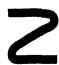
\includegraphics[keepaspectratio]{images/part001_73a6a0da.jpg}}

我们回忆，根据 Ascoli 定理（GT, X, §2, No. 5, Th. 2 的推论 3），\(\mathcal{K}(\mathrm{X};\mathrm{E})\) 的含于 \(\mathcal{K}(\mathrm{X},\mathrm{K};\mathrm{E})\) 中的严格紧子集 H 由下列条件刻画：\(1^{\circ}\) 它是闭的；\(2^{\circ}\) 它是等度连续的；\(3^{\circ}\) 对每个 \(x\in \mathbf{K}\) ，集 \(\mathrm{H}(x)\) 在 E 中相对紧。

推论. --- 设 X 是一个仿紧局部紧空间；若 E 是一个拟完备局部凸空间，则空间 \(\mathcal{K}(X;E)\) 是拟完备的。

根据命题 2, (ii)，只需注意：对 X 的每个紧子集 K，\(\mathcal{K}(X,K;E)\) 是 \(\mathcal{C}(K;E)\) 的一个闭子空间，后者是拟完备的，因为 \(\mathcal{C}(K;E)\) 的每个有界子集都由取值于 E 的同一个有界子集中的函数组成。

